\subsection{The array object}

\begin{frame}
  What makes an array so much faster?
  \begin{itemize}
  \item Data layout
    \begin{itemize}
    \item homogenous: every item takes up the same size block of memory
    \item single data-type objects
    \item powerful array scalar types
    \end{itemize}
  \item universal function (ufuncs)
    \begin{itemize}
    \item function that operates on ndarrays in an element-by-element fashion
    \item vectorized wrapper for a function
    \item built-in functions are implemented in compiled C code
    \end{itemize}
\end{itemize}
\end{frame}

\begin{frame}
  Data layout
  \begin{itemize}
  \item homogenous: every item takes up the same size block of memory
  \item single data-type objects
  \item powerful array scalar types
  \end{itemize}
  \begin{center}
    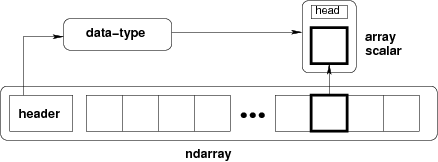
\includegraphics[scale=.5]{../figures/numpy/threefundamental.png}
  \end{center}
\end{frame}

\begin{frame}[fragile]
  universal function (ufuncs)
  \begin{itemize}
  \item function that operates on ndarrays in an element-by-element fashion
  \item vectorized wrapper for a function
  \item built-in functions are implemented in compiled C code
  \end{itemize}
  \begin{block}{python function v ufunc}
    \begin{minted}{python}
In [31]: %timeit [sin(i)**2 for i in arr]
1 loops, best of 3: 4.32 s per loop

In [32]: import numpy as np

In [33]: %timeit np.sin(arr)**2
10 loops, best of 3: 20.8 ms per loop
    \end{minted}
  \end{block}
\end{frame}

\begin{frame}[fragile]
\begin{block}{Creating array}
\begin{minted}{python}
In [5]: x = array([2, 3, 12]) # Create from list

# mix of tuple, lists, and types
In [6]: x = np.array([[1,2.0],[0,0],(1+1j,3.)])

In [7]: x = arange(-10, 10, 2, dtype=float)

In [8]: np.linspace(1., 4., 6)

In [9]: np.indices((3,3))

In [10]: fromfile('foo.dat')
\end{minted}
\end{block}
\end{frame}

\subsection{Array slicing and striding}
\subsection{Other Capabilities}

\begin{frame}[fragile]
\begin{block}{Array API}
\begin{minted}{python}
In [16]: x = arange(9).reshape(3,3)
In [19]: x[:, 0]
Out[19]: array([0, 3, 6])
In [20]: x.shape
Out[20]: (3, 3)
In [21]: x.strides
Out[21]: (24, 8)
In [22]: y = x[::2, ::2]
In [25]: y[0,0] = 100
In [26]: x[0, 0]
Out[26]: 100
\end{minted}
\end{block}
\end{frame}

\begin{frame}[fragile]
Finite Differences
 \begin{block}{computing blocks}
   \begin{minted}{python}
In [38]: x = np.arange(0, 20, 2)

In [40]: y = x**2

In [42]: dy_dx = ((y[1:] - y[:-1]) / (x[1:] - x[:-1]))
In [43]: dy_dx
Out[43]: array([ 2,  6, ... 30, 34])

In [44]: dy_dx_c = ((y[2:] - y[:-2])/(x[2:] - x[:-2]))
In [45]: dy_dx_c
Out[45]: array([ 4,  8, ... 28, 32])
\end{minted}
\end{block}
\end{frame}


